\documentclass[tikz,border=10pt]{standalone}
\usepackage{tikz}
\usetikzlibrary{arrows.meta}
\begin{document}
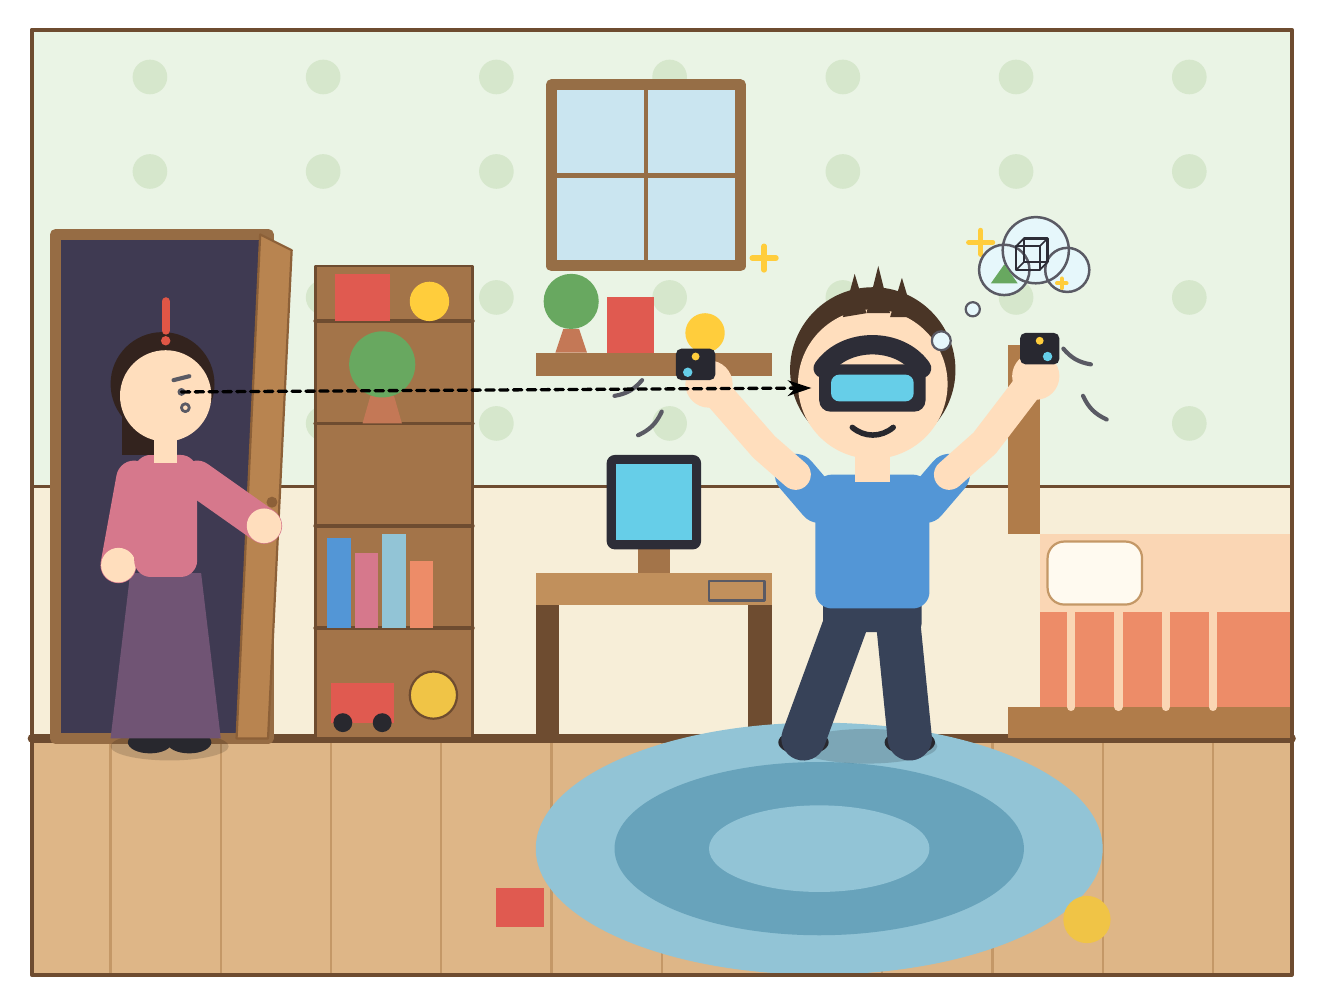
\begin{tikzpicture}[line cap=round, line join=round]

% ================= Palette =================
\definecolor{wallColor}{RGB}{234,244,229}
\definecolor{wallDot}{RGB}{214,231,204}
\definecolor{wainscot}{RGB}{247,238,216}
\definecolor{floorColor}{RGB}{222,182,135}
\definecolor{floorDark}{RGB}{196,152,103}
\definecolor{baseboard}{RGB}{110,76,48}
\definecolor{doorHall}{RGB}{63,58,82}
\definecolor{doorFrame}{RGB}{150,108,68}
\definecolor{doorPanel}{RGB}{184,132,80}
\definecolor{doorPanelDark}{RGB}{140,96,56}
\definecolor{shelfWood}{RGB}{163,116,73}
\definecolor{deskWood}{RGB}{193,144,92}
\definecolor{bedFrame}{RGB}{176,124,74}
\definecolor{bedLinenA}{RGB}{237,140,104}
\definecolor{bedLinenB}{RGB}{250,214,180}
\definecolor{pillowColor}{RGB}{255,250,240}
\definecolor{rugColor}{RGB}{146,196,214}
\definecolor{rugColorDark}{RGB}{104,163,187}
\definecolor{skin}{RGB}{255,222,189}
\definecolor{boyHair}{RGB}{74,53,38}
\definecolor{boyShirt}{RGB}{83,150,214}
\definecolor{boyShorts}{RGB}{55,66,88}
\definecolor{shoeColor}{RGB}{40,40,46}
\definecolor{headsetColor}{RGB}{45,45,55}
\definecolor{headsetLens}{RGB}{102,206,232}
\definecolor{controllerColor}{RGB}{40,40,48}
\definecolor{momHair}{RGB}{51,35,30}
\definecolor{momTop}{RGB}{214,120,140}
\definecolor{momSkirt}{RGB}{112,84,116}
\definecolor{windowFrame}{RGB}{150,110,70}
\definecolor{sky}{RGB}{202,229,240}
\definecolor{plantPot}{RGB}{196,120,86}
\definecolor{plantLeaf}{RGB}{104,168,96}
\definecolor{sparkle}{RGB}{255,205,60}
\definecolor{toyRed}{RGB}{224,90,80}
\definecolor{toyYellow}{RGB}{240,196,70}
\definecolor{bubbleFill}{RGB}{230,247,251}
\definecolor{outline}{RGB}{90,90,100}
\definecolor{exclaimColor}{RGB}{224,86,70}

% ================= Back wall =================
\fill[wallColor] (0,3) rectangle (16,12);
\fill[wainscot] (0,3) rectangle (16,6.2);
\draw[baseboard,line width=1.2pt] (0,6.2) -- (16,6.2);
\foreach \x in {1.5,3.7,...,15.5}{
  \foreach \y in {7.0,8.6,10.2,11.4}{
    \fill[wallDot] (\x,\y) circle (0.22);
  }
}

% window on back wall
\fill[sky] (6.6,9.0) rectangle (9.0,11.3);
\draw[windowFrame,line width=4pt] (6.6,9.0) rectangle (9.0,11.3);
\draw[windowFrame,line width=1.6pt] (7.8,9.0) -- (7.8,11.3);
\draw[windowFrame,line width=1.6pt] (6.6,10.15) -- (9.0,10.15);

% ================= Floor =================
\fill[floorColor] (0,0) rectangle (16,3);
\foreach \x in {1,2.4,...,15}{
  \draw[floorDark,line width=0.8pt] (\x,0) -- (\x,3);
}
\draw[baseboard,line width=3pt] (0,3) -- (16,3);

% ================= Doorway (mother enters here) =================
\fill[doorHall] (0.3,3) rectangle (3.0,9.4);
\draw[doorFrame,line width=4pt] (0.3,3) rectangle (3.0,9.4);
\fill[doorPanel] (2.6,3) -- (3.0,3) -- (3.3,9.2) -- (2.9,9.4) -- cycle;
\draw[doorPanelDark,line width=0.8pt] (2.6,3) -- (3.0,3) -- (3.3,9.2) -- (2.9,9.4) -- cycle;
\fill[doorPanelDark] (3.05,6.0) circle (0.07);

% ================= Bookshelf =================
\fill[shelfWood] (3.6,3) rectangle (5.6,9.0);
\draw[baseboard,line width=1pt] (3.6,3) rectangle (5.6,9.0);
\foreach \y in {4.4,5.7,7.0,8.3}{
  \draw[baseboard,line width=1.4pt] (3.6,\y) -- (5.6,\y);
}
% bottom compartment: toy car + ball
\fill[toyRed] (3.8,3.2) rectangle (4.6,3.7);
\fill[shoeColor] (3.95,3.2) circle (0.12);
\fill[shoeColor] (4.45,3.2) circle (0.12);
\fill[toyYellow] (5.1,3.55) circle (0.3);
\draw[baseboard,line width=0.8pt] (5.1,3.55) circle (0.3);
% books standing
\fill[boyShirt] (3.75,4.4) rectangle (4.05,5.55);
\fill[momTop] (4.1,4.4) rectangle (4.4,5.35);
\fill[rugColor] (4.45,4.4) rectangle (4.75,5.6);
\fill[bedLinenA] (4.8,4.4) rectangle (5.1,5.25);
% small potted plant
\fill[plantPot] (4.2,7.0) -- (4.7,7.0) -- (4.6,7.35) -- (4.3,7.35) -- cycle;
\fill[plantLeaf] (4.45,7.75) circle (0.42);
% stacked box + ball
\fill[toyRed] (3.85,8.3) rectangle (4.55,8.9);
\fill[sparkle] (5.05,8.55) circle (0.25);

% ================= Desk with monitor =================
\fill[deskWood] (6.4,4.7) rectangle (9.4,5.1);
\fill[baseboard] (6.4,3) rectangle (6.7,4.7);
\fill[baseboard] (9.1,3) rectangle (9.4,4.7);
\fill[shelfWood] (7.7,5.1) rectangle (8.1,5.4);
\fill[headsetColor,rounded corners=3pt] (7.3,5.4) rectangle (8.5,6.6);
\fill[headsetLens] (7.42,5.52) rectangle (8.38,6.48);
\draw[outline,line width=1pt] (8.6,4.75) rectangle (9.3,5.0);
% wall shelf above desk
\fill[shelfWood] (6.4,7.6) rectangle (9.4,7.9);
\fill[plantPot] (6.65,7.9) -- (7.05,7.9) -- (6.95,8.2) -- (6.75,8.2) -- cycle;
\fill[plantLeaf] (6.85,8.55) circle (0.35);
\fill[toyRed] (7.3,7.9) rectangle (7.9,8.6);
\fill[sparkle] (8.55,8.15) circle (0.25);

% ================= Bed =================
\fill[bedFrame] (12.4,5.6) rectangle (12.8,8.0);
\fill[bedFrame] (12.4,3) rectangle (16.0,3.4);
\fill[bedLinenB] (12.8,3.4) rectangle (16.0,5.6);
\fill[bedLinenA] (12.8,3.4) rectangle (16.0,4.6);
\foreach \x in {13.2,13.8,...,15.6}{
  \draw[bedLinenB,line width=3pt] (\x,3.4) -- (\x,4.6);
}
\fill[pillowColor,rounded corners=6pt] (12.9,4.7) rectangle (14.1,5.5);
\draw[floorDark,line width=0.8pt,rounded corners=6pt] (12.9,4.7) rectangle (14.1,5.5);

% ================= Rug + floor toys =================
\fill[rugColor] (10.0,1.6) ellipse (3.6 and 1.6);
\fill[rugColorDark] (10.0,1.6) ellipse (2.6 and 1.1);
\fill[rugColor] (10.0,1.6) ellipse (1.4 and 0.55);
\fill[toyRed] (5.9,0.6) rectangle (6.5,1.1);
\fill[toyYellow] (13.4,0.7) circle (0.3);

% ================= Mother (in the doorway) =================
\fill[black,opacity=0.15] (1.75,2.9) ellipse (0.75 and 0.18);
\fill[shoeColor] (1.5,2.95) ellipse (0.28 and 0.14);
\fill[shoeColor] (2.0,2.95) ellipse (0.28 and 0.14);
\fill[momSkirt] (1.25,5.1) -- (2.15,5.1) -- (2.4,3.0) -- (1.0,3.0) -- cycle;
% arm reaching toward the door frame
\draw[momTop,line width=13pt] (2.1,6.3) -- (2.95,5.7);
\fill[skin] (2.95,5.7) circle (0.22);
% arm hanging at side
\draw[momTop,line width=13pt] (1.3,6.3) -- (1.1,5.2);
\fill[skin] (1.1,5.2) circle (0.22);
\fill[momTop,rounded corners=6pt] (1.3,5.05) rectangle (2.1,6.6);
% neck + head
\fill[skin] (1.55,6.5) rectangle (1.85,6.85);
\fill[momHair] (1.15,6.6) rectangle (1.55,7.6);
\fill[momHair] (1.66,7.5) circle (0.66);
\fill[skin] (1.7,7.35) circle (0.58);
% face turned toward the son (right side)
\fill[outline] (1.9,7.4) circle (0.05);
\draw[outline,line width=1.5pt] (1.8,7.55) -- (2.0,7.6);
\draw[outline,line width=1pt] (1.95,7.2) circle (0.05);
% surprise mark above her head
\fill[exclaimColor] (1.7,8.05) circle (0.06);
\draw[exclaimColor,line width=3pt] (1.7,8.18) -- (1.7,8.55);

% ================= Boy (playing VR) =================
\fill[black,opacity=0.15] (10.6,2.9) ellipse (0.9 and 0.22);
% shoes
\fill[shoeColor] (9.8,2.95) ellipse (0.32 and 0.16);
\fill[shoeColor] (11.15,2.95) ellipse (0.32 and 0.16);
% legs
\draw[boyShorts,line width=16pt] (10.35,4.5) -- (9.8,3.0);
\draw[boyShorts,line width=16pt] (11.0,4.5) -- (11.15,3.0);
\fill[boyShorts,rounded corners=3pt] (10.05,4.35) rectangle (11.3,4.9);
% torso
\fill[boyShirt,rounded corners=6pt] (9.95,4.65) rectangle (11.4,6.35);
% arms raised with controllers (dynamic, excited pose)
\draw[boyShirt,line width=15pt] (10.0,6.0) -- (9.7,6.35);
\draw[skin,line width=11pt] (9.7,6.35) -- (9.3,6.7) -- (8.6,7.5);
\fill[skin] (8.6,7.5) circle (0.3);
\fill[controllerColor,rounded corners=2pt] (8.18,7.55) rectangle (8.68,7.95);
\fill[sparkle] (8.43,7.85) circle (0.05);
\fill[headsetLens] (8.33,7.65) circle (0.06);
\draw[outline,line width=1.5pt] (8.0,7.15) to[bend left=20] (7.7,6.85);
\draw[outline,line width=1.5pt] (7.75,7.55) to[bend left=20] (7.4,7.35);

\draw[boyShirt,line width=15pt] (11.35,6.0) -- (11.65,6.35);
\draw[skin,line width=11pt] (11.65,6.35) -- (12.1,6.75) -- (12.75,7.6);
\fill[skin] (12.75,7.6) circle (0.3);
\fill[controllerColor,rounded corners=2pt] (12.55,7.75) rectangle (13.05,8.15);
\fill[sparkle] (12.8,8.05) circle (0.05);
\fill[headsetLens] (12.9,7.85) circle (0.06);
\draw[outline,line width=1.5pt] (13.35,7.35) to[bend right=20] (13.65,7.05);
\draw[outline,line width=1.5pt] (13.1,7.95) to[bend right=20] (13.45,7.75);

% neck + head
\fill[skin] (10.45,6.25) rectangle (10.9,6.7);
\fill[boyHair] (10.68,7.68) circle (1.05);
\fill[skin] (10.68,7.5) circle (0.95);
\fill[boyHair] (10.3,8.35) -- (10.45,8.9) -- (10.6,8.4) -- cycle;
\fill[boyHair] (10.6,8.4) -- (10.75,9.0) -- (10.9,8.4) -- cycle;
\fill[boyHair] (10.9,8.35) -- (11.05,8.85) -- (11.2,8.35) -- cycle;
% headset covering the eyes
\fill[headsetColor,rounded corners=4pt] (10.0,7.15) rectangle (11.35,7.75);
\fill[headsetLens,rounded corners=3pt] (10.15,7.28) rectangle (11.2,7.62);
\draw[headsetColor,line width=7pt] (10.05,7.7) to[bend left=55] (11.3,7.7);
% big happy grin
\draw[shoeColor,line width=2pt] (10.42,6.95) to[bend right=40] (10.94,6.95);

% sparkles of excitement around him
\draw[sparkle,line width=2pt] (9.15,9.1) -- (9.45,9.1);
\draw[sparkle,line width=2pt] (9.3,8.95) -- (9.3,9.25);
\draw[sparkle,line width=2pt] (11.9,9.3) -- (12.2,9.3);
\draw[sparkle,line width=2pt] (12.05,9.15) -- (12.05,9.45);

% ---- thought bubble: the virtual world he actually sees ----
\fill[bubbleFill] (11.55,8.05) circle (0.12);
\draw[outline,line width=0.8pt] (11.55,8.05) circle (0.12);
\fill[bubbleFill] (11.95,8.45) circle (0.09);
\draw[outline,line width=0.8pt] (11.95,8.45) circle (0.09);
\fill[bubbleFill] (12.35,8.95) circle (0.32);
\fill[bubbleFill] (12.75,9.2) circle (0.42);
\fill[bubbleFill] (13.15,8.95) circle (0.28);
\draw[outline,line width=0.9pt] (12.35,8.95) circle (0.32);
\draw[outline,line width=0.9pt] (12.75,9.2) circle (0.42);
\draw[outline,line width=0.9pt] (13.15,8.95) circle (0.28);
% little game doodle inside the bubble: wireframe cube + star + mountain
\draw[headsetColor,line width=0.8pt] (12.5,8.95) rectangle (12.8,9.25);
\draw[headsetColor,line width=0.8pt] (12.6,9.05) rectangle (12.9,9.35);
\draw[headsetColor,line width=0.6pt] (12.5,8.95) -- (12.6,9.05);
\draw[headsetColor,line width=0.6pt] (12.8,8.95) -- (12.9,9.05);
\draw[headsetColor,line width=0.6pt] (12.8,9.25) -- (12.9,9.35);
\draw[headsetColor,line width=0.6pt] (12.5,9.25) -- (12.6,9.35);
\fill[plantLeaf] (12.18,8.78) -- (12.35,9.02) -- (12.52,8.78) -- cycle;
\draw[sparkle,line width=1.5pt] (13.02,8.78) -- (13.14,8.78);
\draw[sparkle,line width=1.5pt] (13.08,8.72) -- (13.08,8.84);

% ================= Gaze relationship =================
% mother watches her son closely
\draw[black,densely dashed,line width=1.2pt,-{Stealth[length=3mm,width=2mm]}]
  (1.9,7.4) -- (9.9,7.45);

% outer frame
\draw[baseboard,line width=1.5pt] (0,0) rectangle (16,12);

\end{tikzpicture}
\end{document}
